\documentclass[12pt]{article}
\renewcommand{\familydefault}{\sfdefault}
\usepackage{lmodern}


\addtolength{\oddsidemargin}{-.975in}
	\addtolength{\evensidemargin}{-.975in}
	\addtolength{\textwidth}{1.75in}

	\addtolength{\topmargin}{-.975in}
	\addtolength{\textheight}{1.75in}

\usepackage[utf8]{inputenc}
\usepackage[hyphens]{url}
\usepackage{float}
\usepackage{amsmath}
\usepackage{latexsym}
\usepackage[portuguese]{babel}
\usepackage{graphicx}
\usepackage{amssymb}
\usepackage{natbib}
\def\ee{\varepsilon}
\def\R{\mathbb R}


\newtheorem{definicao}{Defini\c c\~ao}
\newtheorem{definicao_}{Defini\c c\~ao}
\newtheorem{propriedade_}{Propriedade}
\newtheorem{lema}[definicao]{Lema}%[section]
\newtheorem{proposicao}[definicao]{Proposi\c c\~ao}%[section]
\newtheorem{observacoes}[definicao]{Observações}%[section]
\newtheorem{obs}[definicao]{Observação}%[section]
\newtheorem{observacao}[definicao]{Observação}%[section]
\newtheorem{teorema}[definicao]{Teorema}%[section]
\newtheorem{teointro}{Teorema}%[section]
\newtheorem{conjectura}{Conjectura}%[section]
\newtheorem{corolario}[definicao]{Corol\'ario}%[section]
\newtheorem{exemplo}[definicao]{Exemplo}%[section]
\newtheorem{exemplo_alg}[definicao]{Exemplo}%[section]
\newtheorem{exemplos}[definicao]{Exemplos}%[section]

\def\C{\mathbb C}
\def\Z{\mathbb Z}
\def\N{\mathbb N}
\def\Q{\mathbb Q}
\def\H{\mathbb H}
\def\F{{\mathbb F}_q}
\def\cc{{\mathcal C}}
\def\bv{{\bf v}}
\def\rr{{\mathcal R}_n}
\def\im{{\bf i}}
\def\supp{\mathop{{\rm supp}}}
\def\zen{\mathop{\mathcal{Z}}}
\def\base{\mathcal{B}}
\def\Geny{\mathcal{G}}
\def\vezes{\mathop{{\rm times}}}
\def\Gal{\mathop{{\rm Gal}}}
\def\alge{\mathcal{A}}
\def\pr{\noindent{\sc proof. }}
\def\wh{\widehat}

%\def\lhd{\vartriangleleft}
%\newcommand{\fim}{\hspace*{\fill} $\square$\medskip}
%\newcommand{\ndv}{ \ {\mid \kern -0.70 em {\scriptstyle \not}} \ \ }

\newcommand{\rn}[1]{\mathbb{R}^{#1}}
\newcommand{\xpt}[1]{\dot{#1}}
\newcommand{\en}[1]{\textbf{e}_#1}
\newcommand{\zz}{\mathbb{Z}_{2}}
\newcommand{\dd}{\mathbb{D}_{4}}
\newcommand{\bq}{\begin{equation}}
\newcommand{\e}{\varepsilon}
\newcommand{\T}{\theta}
\newcommand{\f}{\phi}
\newcommand{\eq}{\end{equation}}


%\hyphenation{adapta-dos,mathe-ma-ti-ca,exem-plo,apro-fun-dar,es-tu-dan-te,ma-te-ma-ti-ca}

\pagenumbering{arabic}


%%%%%%%%%%%%%%%%%%%%%%%%%%%% corpo
%%%%%%%%%%%%%%%%%%%%%%%%%%%% %%%%%%%%%%%%%%%%%%%%%%%%%%%%%%%%%%%%%%%%%%%%%%%%%%%%%%%%

%\usepackage{refcheck}
\begin{document}

\fontsize{14}{18} \selectfont 


\begin{center}
{\bf IMECC/Unicamp}\\
{\bf Reltório Parcial de Pesquisa de Iniciação Científica}\\

\vspace{.5cm}

{\bf\Large Métodos numéricos em equações diferenciais suaves por partes em dimensão 2}
\end{center}

\vspace{1cm}

\noindent{\bf Orientador:} Dr. Ricardo Miranda Martins\\
\noindent{\bf Estudante:}  Gabriel Belém Barbosa\\

\medskip
 
\noindent{\bf Enquadramento do projeto em área essencial:} Pesquisa Básica.

\noindent{\bf Palavras-chave:} Equações diferenciais, sistemas de Filippov, órbitas periódicas.


\section*{Resumo das atividades}
\subsection*{Objetivos completos}
Este projeto visa estudar equações diferenciais suaves por partes de um ponto de vista numérico, em especial o estudo de soluções periódicas para sistemas de equações diferenciais lineares por partes em dimensão 2 no caso em que a região de
descontinuidade é regular. Até o presente momento foi estudado em particular a existência (e quantidade) de ciclos limite e a formação destes sob pequenas perturbações. Os principais textos base foram \cite{Huan:etal:2012}, que trata de investigar o número de ciclos limite em um sistema de equações diferenciais lineares e planares através do estudo do comportamento do mapa de retorno de Poincaré em casos específicos, e \cite{HAN20102399}, que trata do fenômeno de bifurcação de Hopf nesses mesmos sistemas com forte emprego de estratégias comuns no estudo local de perturbações de sistemas dinâmicos. Além disso foi empregado material auxiliar para obter-se mais aprofundamento no tema de Bifurcação de Hopf em \cite{Kuznetsov:1998} e para aplicar teoria de garantia de convergência do método de Newton para a demonstração da existência de ciclos limites em \cite{LilPonce2012} e \cite{Tapia1971}. No projeto foram produzidos diversos exemplos de sistemas dinâmicos com comportamentos conhecidos (tanto não-perturbados quanto  perturbados), além da elaboração de exemplos (e de um método geral para a obtenção de exemplos) de um sistema com 3 ciclos limite.





Objetivos específicos iniciais do projeto são:

\begin{enumerate}
\item Estudar a convenção de Filippov para soluções de equações diferenciais suaves por partes.
\item Estudar os artigos \cite{Huan:etal:2012} e \cite{LilPonce2012}.
\item Produzir exemplos de sistemas com pelo menos 3 ciclos limite, como feito em \cite{Huan:etal:2012}.
\item Estudar o número máximo de ciclos limite que podem ser obtidos com sistemas de equações diferenciais lineares por partes, com superfície de descontinuidade $xy=0$.
\end{enumerate}
Dos quais foram cumpridos os 3 primeiros.
\subsection*{Cronograma e produção científica}
\noindent {\bf Setembro/2021:} Revisar sistemas de equações diferenciais lineares planares..\\

\noindent {\bf Outubro-novembro/2021}: Estudar os conceitos básicos da convenção de Filippov.\\

\noindent {\bf Dezembro/2021-janeiro/2022}: Estudar o artigo \cite{Huan:etal:2012}.\\

\noindent {\bf Fevereiro/2022}: Elaboração do relatório parcial.\\

\noindent {\bf Março/2022}: Estudar o artigo \cite{LilPonce2012}.\\

\noindent {\bf Abril/2022}: Produzir novos exemplos de equações diferenciais suaves por partes com 3 ciclos limite.\\

\noindent {\bf Maio/2022}: Estudar o problema da existência de ciclos limite em sistemas de equações diferenciais lineares por partes, com superfície de descontinuidade $xy=0$.\\

\noindent {\bf Junho-julho/2022}: Realizar simulações computacionais e obter exemplos, com o objetivo de estabelecer uma conjectura sobre o número máximo de ciclos limite (no caso anterior).\\

\noindent {\bf Agosto/2022}: Elaborar o relatório final.\\

Até o presente momento foram cumpridas até as atividades propostas  referentes ao mês de abril do cronograma inicial. Nos próximos seis meses, 


O projeto foi utilizado como base para a matéria Projetos Supervisionados (MS777) do Instituto de Matemática Aplicada e Computacional  da Unicamp, que conta com a produção de uma monografia e uma apresentação de 10 minutos explorando seu conteúdo, além de dez minutos adicionais para perguntas e respostas com o aluno. O material produzido, monografia e apresentação, receberam a segunda melhor avaliação da bancada de professores jurados, e podem ser encontrados no link:

\begin{center}\url{https://www.ime.unicamp.br/~mac/galeria.html}\end{center}

No projeto foram produzidos diversos exemplos de sistemas dinâmicos com comportamentos conhecidos (tanto não-perturbados quanto  perturbados), além da elaboração de exemplos (e de um método geral para a obtenção de exemplos) de um sistema com 3 ciclos limite.

\section*{Resultados obtidos}


Com uma transformação para a forma de Jordan, os sistemas estudados podem ser escritos na forma
\begin{equation}
\label{eqn:jor}
\dot{\mathbf{x}}=\left\{\begin{array}{ll}
\mathbf{J}^{+} \mathbf{x} & \text { se } x \geq 1 \\
\mathbf{A}^{-} \mathbf{x} & \text { se } x<1
\end{array},\text{ }\mathbf{x}=\begin{pmatrix}
x\\
y
\end{pmatrix}\right.,
\end{equation}
sendo $\mathbf{J}^{+}$ a forma normal de Jordan de $\mathbf{A}^{+}$,
\[
\mathbf{J}^{+}=\left(\begin{array}{cc}
\alpha^{+} & -\beta^{+} \\
\beta^{+} & \alpha^{+}
\end{array}\right).
\]

Utilizando o método descrito em detalhes na monografia, que envolve a análise e manipulações sucessivas com métodos numéricos dos mapas de retorno de cada subsistema, mais um ajuste manual de alguns parâmetros, dado um sistema linear repulsor para o lado direito da linha de corte, foi obtido um sistema na forma (\ref{eqn:jor}) que possui 3 ciclos limites, com
\[
A^+=
\begin{pmatrix}
\frac{3}{4}& -1\\
1& \frac{3}{4}
\end{pmatrix}
\]
a forma de Jordan normalizada em $\beta^-$ do subsistema direito (com $\gamma^+=0.75$) e
\[
A^-=
\begin{pmatrix}
13.43538491431723& -18.14977774439898\\
10.01439047867205& -13.50150142642550
\end{pmatrix},
\]

Uma solução periódica de \ref{eqn:jor} pode ser descrita como a solução $(t^+, t^-, Y)$ do sistema
\begin{align}
\label{u}
&u_{1}\left(t^{+}, t^{-}, Y\right)=x^{+}\left(-t^{+}\right)-1=0 \nonumber\\
&u_{2}\left(t^{+}, t^{-}, Y\right)=x^{-}\left(t^{-}\right)-1=0 \\
&u_{3}\left(t^{+}, t^{-}, Y\right)=y^{+}\left(-t^{+}\right)-y^{-}\left(t^{-}\right)=0\nonumber.
\end{align}

Foi provado que o sistema (\ref{u}) das matrizes $A^-$ e $A^+$ apresentadas possui soluções próximas à

$$\begin{array}{l|l|l}
t^+_1 = 0.060050041701417& \ \ \ t^+_2 = 0.090075062552126&t^+_3 = 0.225187656380317\\
t^-_1 = 7.536280233527940& \ \ \ t^-_2 = 6.755629691409507&t^-_3 = 5.899916597164303\\
Y_1 = 0.791849893551496& \ \ \ Y_2 = 0.820743212919858&Y_3 = 0.928334461670545
\end{array}$$

Para tal, foi usado o método presente em \cite{LilPonce2012}, no qual mais detalhes sobre como achar os limitantes de algumas normas estão presentes, que aqui serão omitidos por brevidade. A base da prova está no teorema de Newton-Kantorovich e pode ser acompanhada na monografia.

Na Figura \ref{triz} os três ciclos limites do sistema podem ser observados.

\begin{figure}[H]
\centering
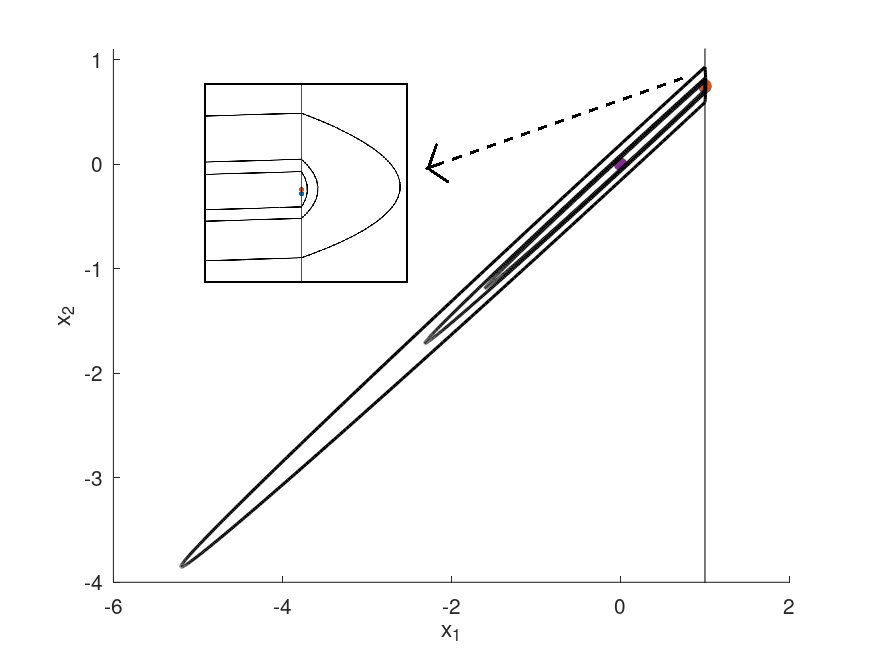
\includegraphics[width=10cm]{triz}\\
\vspace{\baselineskip}
\caption{\label{triz}Três ciclos limite a partir de $\gamma^+=0.75$.}
\end{figure}
Além disso foi estudado o fenômeno de bifurcação de Hopf em \cite{Kuznetsov:1998} de forma geral e em particular no âmbito dos sistemas em foco, obtendo-se sistemas com comportamentos distintos por meio da variação de certos parâmetros através de pontos críticos, como descrito em \cite{HAN20102399}. Com mais detalhes na monografia, um sistema sem ciclos limites (Figura \ref{undist}) foi levado a um com somente um ciclo limite (Figura \ref{hdist}) e depois foi formado um segundo ciclo limite com estabilidade contrária no interior deste primeiro (Figura \ref{dist}, na qual as cores representam a mudança d estabilidade, que depende do sentido do sistema).
\begin{figure}[H]
\centering
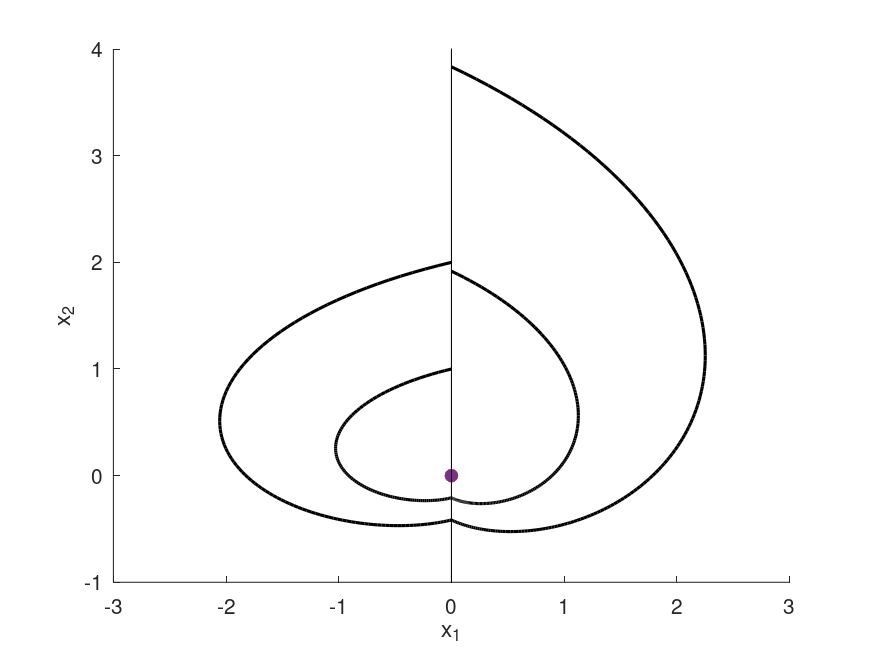
\includegraphics[width=9cm]{disturb_pre}\\
\caption{\label{undist}$b^\pm=\vec{0}$}
\end{figure}

\begin{figure}[H]
\minipage{0.45\textwidth}
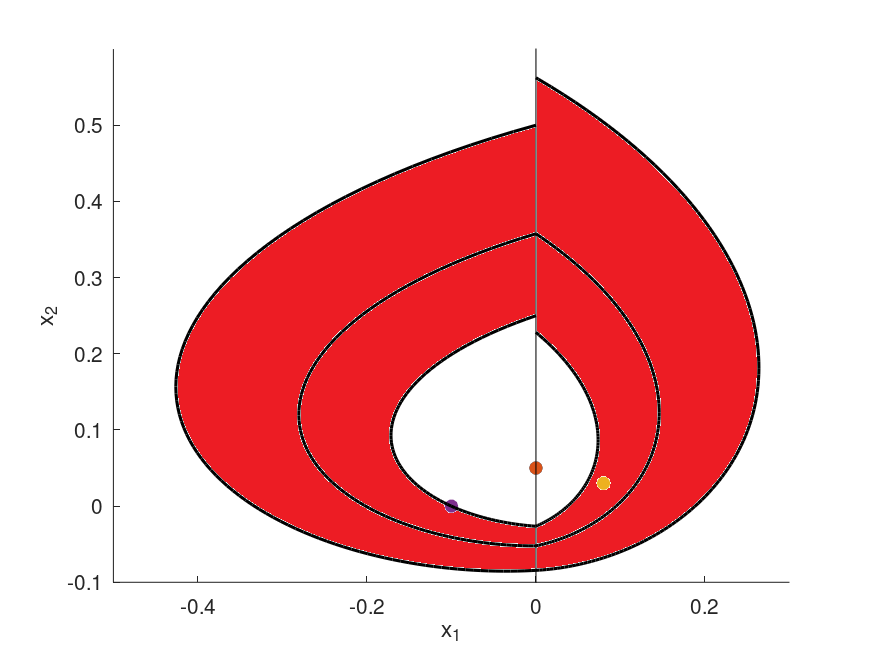
\includegraphics[width=\linewidth]{disturb_mid}\\
\caption{\label{hdist}$\left|b_{1}^{\pm}\right|+\left|b_{2}^{\pm}\right|<\varepsilon_{0},\text{ }0<\varphi_{1}\left(b_{1}^{+}\right)-b_{1}^{-} \ll 1,\text{ }b_{2}^{+}<\varphi_{3}\left(b_{1}^{+}\right),\text{ }  \varphi_{2}\left(b_{1}^{+}\right)<b_{2}^{-}<\tilde{\varphi}\left(b_{1}^{+}, b_{2}^{+}\right).$}
\endminipage
\hspace{0.1\textwidth}
\minipage{0.45\textwidth}
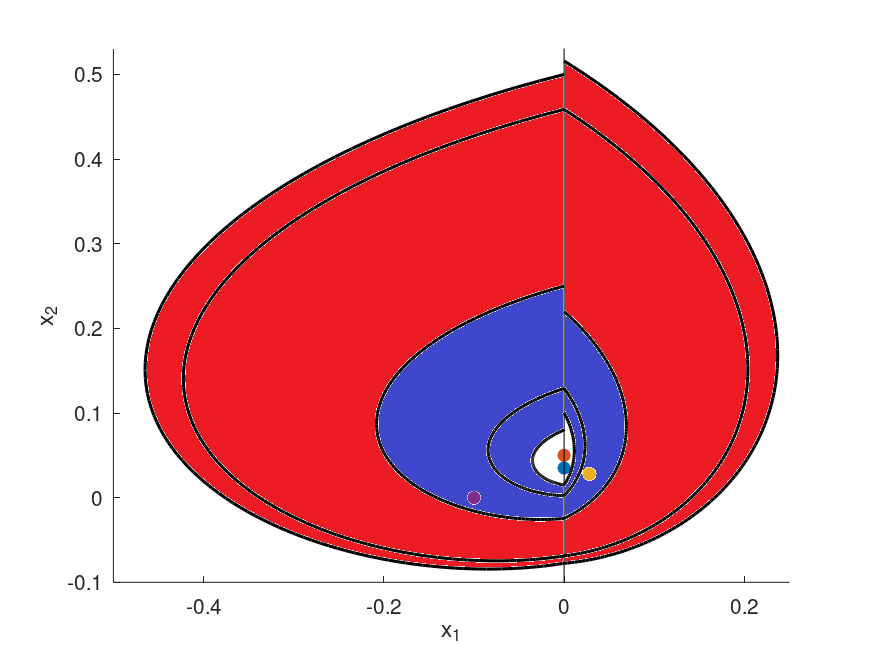
\includegraphics[width=\linewidth]{disturb_pos}\\
\caption{\label{dist}$\left|b_{1}^{\pm}\right|+\left|b_{2}^{\pm}\right|<\varepsilon_{0},\text{ }0<b_{1}^{-}-\varphi_{1}\left(b_{1}^{+}\right) \ll 1,\text{ }b_{2}^{+}<\varphi_{3}\left(b_{1}^{+}\right),\text{ }  \varphi_{2}\left(b_{1}^{+}\right)<b_{2}^{-}<\tilde{\varphi}\left(b_{1}^{+}, b_{2}^{+}\right).$}
\endminipage
\end{figure}

\bibliographystyle{plainnat}
\bibliography{monografia}



\bigskip

\bigskip

Campinas, \today

\end{document}
